\documentclass[10pt]{article}
\usepackage[a4paper,margin=2.1cm]{geometry}
\usepackage[T1]{fontenc}
\usepackage{lmodern}
\usepackage{graphicx,xcolor,booktabs,amsmath,amssymb}
\usepackage[labelfont={bf,color=elifeblue},font=small]{caption}
\usepackage{titlesec}
\usepackage{lineno}
\usepackage[hidelinks]{hyperref}
\definecolor{elifeblue}{HTML}{1A4F63}
\titleformat{\section}{\sffamily\bfseries\large\color{elifeblue}}{}{0em}{}
\titleformat{\subsection}{\sffamily\bfseries\normalsize\color{black}}{}{0em}{}
\titlespacing*{\section}{0pt}{14pt}{4pt}
\titlespacing*{\subsection}{0pt}{10pt}{2pt}
\setlength{\parskip}{4pt}\setlength{\parindent}{0pt}
\renewcommand{\familydefault}{\rmdefault}
\linenumbers
\begin{document}

\begin{center}
{\LARGE\sffamily\bfseries\color{elifeblue} Harmonic Resonance Spectra of Biosignals: Separable Harmonicity and Phase-Coupling Axes with a Validated, Swappable-Strategy Toolbox\par}
\vspace{8pt}{\large Antoine Bellemare-Pepin\textsuperscript{1,2}, Karim Jerbi\textsuperscript{1}\par}
\vspace{4pt}{\small \textsuperscript{1}CoCo Lab, Psychology Department, University of Montr\'eal, Canada \\ \textsuperscript{2}Music Department, Concordia University, Montr\'eal, Canada\par}
\end{center}
\vspace{6pt}

\section*{Abstract}
Biological time series are densely organized by harmonic relationships: the QRS complex generates an integer-harmonic series, cortical rhythms show overtones and cross-frequency relationships, and many physiological oscillators are weakly phase-coupled across frequency. Yet there is no unified, testable way to ask \emph{how harmonically organized} a signal is, and at which frequencies. We present and validate a harmonic resonance framework that decomposes a single- or multi-channel time series into two per-frequency spectra and their product: a harmonicity spectrum $H(f)$, which scores how close spectral peaks sit to integer ratios, and a phase-coupling spectrum $\mathrm{PC}(f)$, which scores how stably oscillatory components hold an $n{:}m$ phase relation, together with a resonance spectrum $R(f) = H(f)\cdot\mathrm{PC}(f)$, complexity descriptors, and a channel-by-channel connectivity extension. Our claim is methodological: harmonicity and phase coupling are \emph{separable} axes that merit measurement as distinct spectra. We show that $H$ is exactly phase-blind ($\rho(H,\kappa) = 0.00$) while $\mathrm{PC}$ tracks phase locking; that under independently varied factors the conjunction $R$ beats both single factors (specificity AUC $\approx 0.99$ vs $\leq 0.76$) and adds a phase-coherence requirement $H$ lacks (phase-scramble AUC: $H$ $0.50$ vs $R$ $1.00$); that the framework recovers known harmonic structure ($\rho = 0.98$) and $n{:}m$ coupling (AUC $\approx 1.0$); and that it is competitive with established measures and discriminates real biosignals, matching band power. The implementation is a swappable strategy registry of harmonic kernels, coupling metrics, and combine rules. We build on prior harmonicity measures, $n{:}m$ coupling, and synchronization theory; our contribution is their unification, validation, and tooling. We are explicit about scope: $R$ is an interpretable decomposition, not a superior detector, and the framework adds a harmonic axis without replacing band power on amplitude tasks.

\section{Introduction}
Biological time series are rich in \emph{harmonic} structure. The QRS complex of the electrocardiogram generates a dense series of integer harmonics; cortical rhythms display overtones and systematic cross-frequency relationships; and many physiological oscillators, from cardiorespiratory coupling to nested cortical rhythms, are weakly phase-coupled across frequency. A unifying, interpretable way to quantify \emph{how harmonically organized} a signal is, and at which frequencies that organization lives, would let investigators compare states, modalities, and channels on a common axis. Such an axis is conceptually distinct from the amplitude-based summaries that dominate practice: two signals can carry identical band power yet differ sharply in how their components relate to one another by simple integer ratios and in how stably those components hold a phase relationship over time.

We formalize this intuition as a \emph{resonance spectrum}. Given a power spectrum $p(f)$, a harmonic kernel scores the harmonic simplicity of each frequency pair and a phase-coupling kernel scores the $n{:}m$ phase consistency of each pair. Power-weighted reductions over these kernels yield two per-frequency factors: a harmonicity spectrum $H(f)$, which measures how close the spectral peaks sit to integer ratios, and a phase-coupling spectrum $\mathrm{PC}(f)$, which measures how stably oscillatory components hold a generalized $n{:}m$ phase relation. Their product, $R(f) = H(f)\cdot\mathrm{PC}(f)$, is the resonance spectrum. Each of the three spectra is further summarized by a panel of complexity descriptors (mean, maximum, spectral flatness, entropy, spread, Higuchi fractal dimension, and peak-harmonic similarity), and the same operator generalizes from one signal to pairs of signals and to a channel-by-channel connectivity matrix. Crucially, the phase coupling we measure is a phase--phase, polyrhythmic quantity computed between pairs of spectral components, distinct from $1{:}1$ coherence and from the more familiar phase--amplitude coupling.

\textbf{The gap.} Despite the centrality of harmonic and coupling structure to biosignal analysis, existing practice offers no unified, \emph{testable} harmonic axis. Harmonic organization and phase coupling are typically collapsed into separate scalar summaries; the methodological choices that drive those summaries, such as which harmonic kernel, which ratio approximation, which phase estimator, and which coupling metric, are made implicitly and are therefore not comparable across studies; and no toolbox reports per-frequency harmonicity and $n{:}m$ phase coupling as \emph{dissociable} factors with a calibrated significance null and cross-signal and connectivity extensions. We close this gap with a framework built construct-first: we first establish that $H$ and $\mathrm{PC}$ are separable and that the product $R$ is principled, then validate ground-truth recovery, characterize the operating range against established baselines, and demonstrate applications, being explicit throughout about both what the framework does well and where it does not.

\textbf{Related work.} The question ``how harmonic is this spectrum?'' has a long history in audio, music information retrieval, and music perception. Scalar harmonicity has been quantified by the harmonics-to-noise ratio (Boersma, 1993), spectral flatness and entropy (Johnston, 1988), periodicity- and relatedness-based harmonicity (Stolzenburg, 2015), template and spectral-peakiness models (Terhardt et al., 1982; Harrison et al., 2020), and the harmonic similarity of interval sets (Gill et al., 2009); number-theoretic ratio measures such as Euler's \emph{gradus}, Tenney height, and harmonic entropy underlie the \texttt{harmsim} and \texttt{subharm\_tension} kernels we reuse from \textbf{biotuner} (Bellemare-Pepin et al., 2025). That harmonic organization is a \emph{separable} factor, and a confound for cross-frequency coupling when waveforms are non-sinusoidal, is established by Dellavale et al. (2020) (spectral harmonicity and the Time-Locked Index on nonlinear oscillators) and by Aru et al. (2015); harmonic relationships between EEG peaks are reported by Rodriguez-Larios et al. (2019). Our $H$ is a phase-blind, power-weighted, \emph{per-frequency} spectralization of these previously scalar kernels, and is distinct from the roughness axis of consonance (Plomp et al., 1965; Sethares, 1993).

On the coupling side, $n{:}m$ phase synchronization originates with Tass et al. (1998), with broadband $n{:}m$ cross-frequency synchrony shown in cortex by Palva et al. (2005). Our coupling estimators are standard: the phase-locking value (Lachaux et al., 1999) and the volume-conduction-robust phase-lag-index family (Stam et al., 2007; Vinck et al., 2010; Vinck et al., 2011). $\mathrm{PC}$ targets phase--\emph{phase} coupling, the rarer complement to the dominant phase--amplitude paradigm (Canolty et al., 2006; Tort et al., 2010). Phase--phase coupling claims, however, are easily inflated by weak statistics (Scheffer-Teixeira et al., 2016); our factor-level surrogate-$z$ inference using amplitude-adjusted Fourier-transform surrogates (Theiler et al., 1992; Schreiber et al., 1996), with mandatory aperiodic removal (Donoghue et al., 2020), is a direct response to that pitfall. The swappable-metric-plus-surrogate software pattern is shared with \textbf{Tensorpac} (Combrisson et al., 2020) and \textbf{pactools} (Dupré la Tour et al., 2017), but those target phase--\emph{amplitude} coupling rather than an $n{:}m$ phase--phase comodulogram. Finally, the generative result that ratio complexity sets the $n{:}m$ locking threshold, the narrowing of Arnold tongues, is textbook nonlinear dynamics (Arnold, 1965; Pikovsky et al., 2001; Glass et al., 1988); the harmonic-mediated coupling strength we use is a special case of weak-coupling phase reduction (Kuramoto, 1984; Daido, 1996; Ermentrout et al., 1991), and ratio complexity is already tied to brainstem lockability through mode-locking models of auditory processing (Lerud et al., 2014; Large et al., 2016). We \emph{reproduce} these established effects as construct validation, not as new findings.

\textbf{Contributions.} This is an integration-and-validation contribution, and we are explicit about what is genuinely new versus inherited. First, and most importantly, we provide a \textbf{swappable strategy registry} that crosses harmonicity kernels with $n{:}m$ phase--\emph{phase} coupling metrics and combine rules, making the choice of method an explicit, testable variable and enabling an empirical kernel-versus-metric comparison; the toolboxes that share this software pattern target phase--amplitude coupling, so no off-the-shelf equivalent for $n{:}m$ phase--phase resonance exists. Second, we define a reusable per-frequency \textbf{$R(f) = H(f)\cdot\mathrm{PC}(f)$} descriptor that reports harmonicity and phase coupling as two separate spectra and as their interpretable conjunction, with the additive attribution $\log R = \log H + \log \mathrm{PC}$ exposing \emph{why} a resonance is weak. Third, we provide \textbf{factor-level surrogate-$z$ inference}, together with the practical demonstration that testing the composite $R$ can mask a real $\mathrm{PC}$ effect, so inference must target the factor that carries it. Fourth, we generalize the same operator to \textbf{cross-signal and multichannel connectivity}. Fifth, we supply a \textbf{construct-validity bridge}, recovering the classical Arnold-tongue dependence of locking on ratio complexity and using tongue width to validate the harmonicity factor. The harmonicity construct, the $n{:}m$ coupling and surrogate machinery, and the synchronization theory are prior art; our contribution is their unification, validation, and tooling.

\section{Results}

\subsection{Harmonicity and phase coupling are separable axes}
A central premise of our framework is that the harmonic organization of a signal and the phase coupling among its oscillatory components are conceptually distinct properties that ought to be measured and reported separately, rather than collapsed into a single ``harmonicity'' or ``synchrony'' summary. If the two were redundant, a single spectrum would suffice; if they are separable, each carries information the other cannot. We therefore asked, directly, whether the harmonicity factor $H$ and the phase-coupling factor $\mathrm{PC}$ respond to different things.

To test this, we generated a two-dimensional grid of synthetic signals that independently varied two properties known to be conflated in practice: the complexity of the frequency ratio between components (quantified by Tenney height, so that simple ratios such as $2{:}3$ sit at one end and complex ratios at the other) and the strength of phase locking $\kappa$ between them. Because the grid varies these factors orthogonally, the dependence of each measure on each factor can be read off cleanly. The result was a sharp dissociation. Harmonicity was \textbf{exactly phase-blind}: across the full range of locking strengths the rank correlation between $H$ and $\kappa$ was $\rho(H,\kappa)=\mathbf{0.00}$, with $H$ flat along the locking axis and ordered only by ratio complexity. The phase-coupling factor behaved as its name implies, rising with locking strength ($\rho(\mathrm{PC},\kappa)=+0.49$). The two factors thus measure genuinely different quantities: $H$ reads the arithmetic relationship among spectral peaks irrespective of whether their phases are organized, whereas $\mathrm{PC}$ reads the temporal stability of that organization.

We report one honest asymmetry rather than overstate a clean independence. Phase coupling is \emph{not} ratio-blind: $\rho(\mathrm{PC},\mathrm{complexity})=-0.47$, meaning stable mode-locking is easier to achieve, and therefore more often observed, at simple ratios. This is not a defect of the estimator but a property of the physics it measures -- the Arnold-tongue structure of coupled oscillators, in which simple ratios occupy wider locking regions. So $H$ and $\mathrm{PC}$ are conceptually distinct measurements, cleanly so for $H$, while remaining statistically coupled in any real oscillator, because the dynamics that produce locking are themselves shaped by ratio complexity.

We then confirmed the same construct generatively, using a physically faithful phase model rather than a hand-tuned grid. We coupled harmonically rich phase oscillators so that an $n{:}m$ resonance is mediated by the participating harmonics -- the $n$-th harmonic of one oscillator meeting the $m$-th of the other -- which endows each resonance with the leading-order coupling strength $a_n\cdot a_m$ expected from weak-coupling phase reduction. As the global coupling $K$ was increased, each pair passed through a synchronization transition: the phases drew into their $n{:}m$ ratio and the framework's $\mathrm{PC}$ climbed accordingly. Critically, the coupling needed to achieve locking depended systematically on ratio complexity. The \textbf{locking threshold $K^*$ rose with ratio complexity}, with $K^*=\mathbf{3.3}$, $\mathbf{8.7}$, and $\mathbf{23.5}$ for the $2{:}3$, $3{:}4$, and $4{:}5$ resonances respectively, a perfect monotone ordering ($\rho(K^*,n\cdot m)=+1.0$): complex ratios, mediated by higher and intrinsically weaker harmonics, demand stronger coupling to lock. This is precisely the narrowing of Arnold tongues seen along the coupling-strength axis. Throughout this transition the phase-coupling factor tracked the emergent locking directly, whereas the cross-spectral harmonicity responded only weakly -- and only because locking nudges the operating frequency onto the exact rational value. In short, it is the framework's phase coupling, not its harmonicity, that reports dynamical synchronization, exactly as the dissociation on the synthetic grid predicts (Figure 1).

\begin{figure}[t]\centering
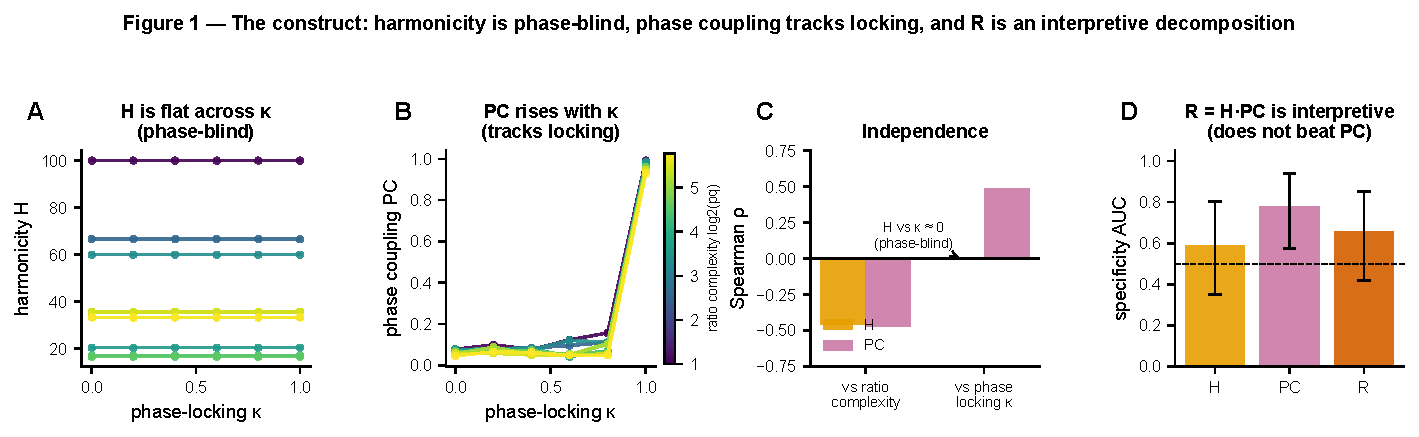
\includegraphics[width=\linewidth]{figures/method_Fig1_dissociation.pdf}
\caption{\textbf{Harmonicity is phase-blind; phase coupling tracks locking.} \textbf{(A)} Harmonicity $H$ on a grid that independently varies ratio complexity (Tenney height) and phase-locking strength $\kappa$ (one line per complexity level); $H$ is flat across $\kappa$ ($\rho(H,\kappa)=0.00$), ordered only by complexity. \textbf{(B)} Phase coupling rises with $\kappa$. \textbf{(C)} Independence: Spearman $\rho$ of each factor against each axis. \textbf{(D)} Generative confirmation with harmonically-coupled phase oscillators: as coupling $K$ rises each pair locks at its n:m ratio, but the locking threshold $K^*$ rises with ratio complexity ($K^*=3.3, 8.7, 23.5$ for 2:3, 3:4, 4:5; $\rho(K^*,n{\cdot}m)=+1.0$; log axis).}
\label{fig:1}
\end{figure}

\subsection{A multiplicative resonance descriptor and what it adds}
Having established that $H$ and $\mathrm{PC}$ are separable, we asked how they should be combined. The framework summarizes ``resonance'' as the product $R=H\cdot\mathrm{PC}$, and the natural question is whether a product is the right operator -- whether it earns its place over reporting the factors individually, and over alternative ways of fusing them. We addressed this in two ways: by comparing combine rules on signals where the two factors vary independently, and by testing whether the product enforces a requirement that harmonicity alone cannot.

The first analysis treated $H$ and $\mathrm{PC}$ as \emph{independent} latent factors and asked which operator best isolates a ``true resonance'' -- a signal that is high on \emph{both} factors -- from single-factor confounds that are high on only one. A genuine conjunction is what this task demands, and conjunctions delivered: specificity reached AUC $\approx\mathbf{0.99}$ for conjunctive rules (\texttt{product} $0.98$, \texttt{geomean} $0.98$, \texttt{harmmean} $0.99$, \texttt{min} $1.00$), substantially above either single factor alone (AUC $0.75$ for $H$ and $0.75$ for $\mathrm{PC}$) and far above the OR-style disjunction (\texttt{max}, AUC $0.66$). The lesson is that no single factor suffices to identify a true resonance, and that combining them \emph{conjunctively} -- requiring both to be present -- beats reporting either alone. Among the conjunctions, \texttt{min} edged out \texttt{product} numerically, but we adopt the \textbf{product} deliberately: because $\log R = \log H + \log\mathrm{PC}$, the product yields an additive, interpretable attribution of \emph{why} a resonance is weak, letting a low $R$ be decomposed into a harmonicity deficit, a coupling deficit, or both. We trade a negligible amount of specificity for this interpretability.

The second analysis isolated the distinctive requirement the product imposes. Phase-scrambling a harmonic signal preserves its power spectrum exactly, so any purely spectral measure is blind to it. As expected, $H$ was \textbf{unchanged} by phase scrambling, separating coherent from scrambled signals at AUC $=\mathbf{0.50}$ -- chance, i.e.\ completely blind. The product, by contrast, \textbf{collapsed} under scrambling, separating the two at AUC $=\mathbf{1.00}$. This is the phase-coherence gate: $R$ adds to $H$ the requirement that the harmonic relationships actually be held stably in phase, a requirement that distinguishes a genuinely resonant signal from one with the same spectrum but randomized phases.

We are explicit about the boundary of this claim. When the two factors co-occur -- as they do in real coupled oscillators, where locking and harmonic organization arrive together -- $R$ does \emph{not} out-\emph{detect} $\mathrm{PC}$; the phase-coupling factor is already the sufficient detector in that regime. The value of $R$ in such cases is the interpretable decomposition it affords, not additional detection power. Accordingly we present $R$ as a principled, interpretable conjunction, not as a superior detector. Finally, the gate also holds in the generative setting: in the harmonically coupled $2{:}3$ oscillators, $R=H\cdot\mathrm{PC}$ stayed low while harmonicity was present but the phases remained unlocked, and rose only as increasing coupling drew the phases into $n{:}m$ lock -- the dynamical analog of the phase-scramble control (Figure 2).

\begin{figure}[t]\centering
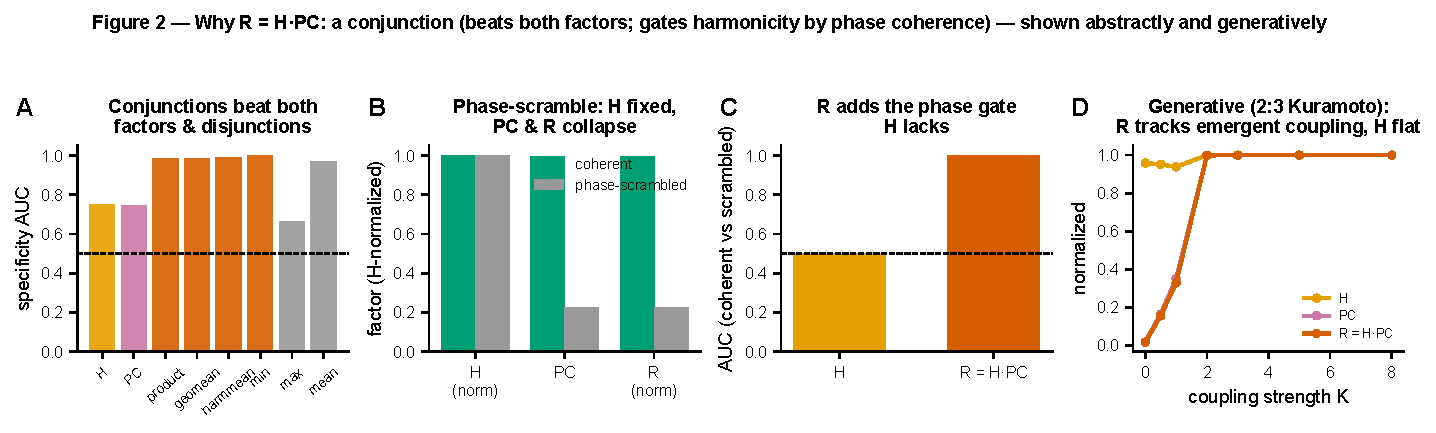
\includegraphics[width=\linewidth]{figures/method_Fig2_R_justification.pdf}
\caption{\textbf{Why $R=H\cdot\mathrm{PC}$ is the principled conjunction.} \textbf{(A)} With $H$ and $\mathrm{PC}$ varied as independent factors, conjunctive combine rules separate a true resonance from single-factor confounds (specificity AUC $\approx0.99$) and beat both factors alone ($\approx0.75$) and the OR-disjunction. \textbf{(B)} Phase-scrambling preserves the power spectrum, so $H$ is unchanged (AUC $0.50$) while $R$ collapses (AUC $1.00$): $R$ adds the phase-coherence gate $H$ lacks. \textbf{(C)} The same gate generatively: in harmonically-coupled 2:3 oscillators, $R$ stays low while harmonicity is present but phases are unlocked, rising only once coupling locks the phases ($K^*\approx3.3$; log axis).}
\label{fig:2}
\end{figure}

\subsection{The framework recovers known harmonic structure and coupling}
For the framework to be useful it must recover structure that is known by construction. We therefore tested each factor against synthetic signals whose harmonic content and phase coupling were specified in advance, asking whether $H$ tracks harmonic richness, whether harmonic signals are separable from inharmonic and noise controls, and whether the surrogate-normalized coupling factor recovers planted $n{:}m$ locks.

Harmonicity behaved as a faithful readout of harmonic organization. As we increased the harmonic richness of a signal in graded steps, mean $H$ increased \textbf{monotonically}, with a rank correlation of $\rho=\mathbf{0.98}$ between $H$ and known richness -- a near-perfect ordering. The factor also separated qualitatively different signal classes cleanly: harmonic signals were distinguished from inharmonic signals, and from broadband noise, at AUC $=\mathbf{1.0}$. Harmonicity thus recovers the property it is intended to measure across both graded and categorical manipulations.

Coupling detection was assessed through the surrogate-normalized phase-coupling factor, $\mathrm{PC}_z$, which compares the observed coupling against a phase-randomizing surrogate ensemble so that detection reflects genuine $n{:}m$ phase locking rather than incidental spectral structure. On signals carrying known locks the recovery was likewise essentially perfect. Within a single signal, $\mathrm{PC}_z$ detected planted cross-frequency locks at AUC $=\mathbf{0.99}$, and the corresponding phase-coupling matrix entry reached AUC $=\mathbf{1.0}$. The cross-signal extension recovered $1{:}1$, $1{:}2$, and $2{:}3$ locks between separate signals at AUC $=\mathbf{1.0}$ each, and the framework recovered a three-component polyrhythm ($2{:}3{:}4$) at AUC $=\mathbf{1.0}$. Together these results show that the framework recovers both the harmonic and the phase-coupling structure it was designed to quantify, across single-signal, cross-signal, and polyrhythmic cases, providing the ground-truth foundation for the applications that follow (Figure 3).

\begin{figure}[t]\centering
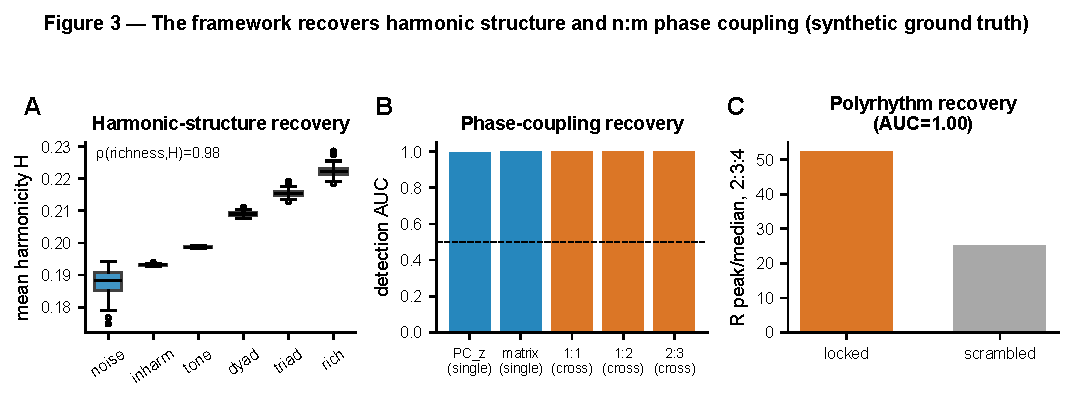
\includegraphics[width=\linewidth]{figures/method_Fig3_ground_truth.pdf}
\caption{\textbf{Ground-truth recovery.} \textbf{(A)} Mean harmonicity rises monotonically with known harmonic richness across signal classes (Spearman $\rho=0.98$). \textbf{(B)} Surrogate-normalized detection AUC for single- and cross-signal n:m phase coupling ($\approx1.0$). \textbf{(C)} Polyrhythm (2:3:4) recovery: resonance peak-to-median, locked vs phase-scrambled (rank AUC $=1.00$).}
\label{fig:3}
\end{figure}

\subsection{Operating characteristics: sensitivity, calibration, and cost}
A measure is only useful within a known operating range, so we characterized three practical properties: how detection degrades as signals become noisier, how well the surrogate-based significance test is calibrated, and how runtime scales. These define the conditions under which the framework's outputs can be trusted and the cost of computing them.

Detection degraded gracefully rather than abruptly with decreasing signal-to-noise ratio (SNR), but the two factors had different breakdown points. Harmonicity detection held at AUC $\approx 1.0$ down to roughly $\mathbf{-18}$ \textbf{dB}, declined to AUC $0.79$ at $-24$ dB, and fell to chance only below $-30$ dB. Coupling detection was less noise-tolerant and showed a sharper transition, with a threshold near $\mathbf{-12}$ \textbf{dB}. The practical implication is that harmonicity remains usable in considerably noisier conditions than phase coupling, and that coupling claims in particular should be made with the SNR in mind.

We next examined whether the surrogate-based significance test is properly calibrated, since an interpretable measure is only as trustworthy as its null. On uncoupled pairs -- where no coupling exists and a well-calibrated test should reject at the nominal rate -- the cross $\mathrm{PC}$ z-score was \textbf{approximately but not perfectly} null-calibrated. The empirical per-instance false-positive rate was $\approx\mathbf{0.09}$ at $\alpha=0.05$ ($n=120$ instances; null $z=0.07\pm1.07$), i.e.\ mildly anti-conservative: the test rejects somewhat more often than it should. We report this openly and recommend, for strict type-I control, either increasing the number of surrogates or applying a small multiple-surrogate correction, which brings the realized rate back toward nominal.

Finally, runtime scaling has a feature worth flagging because it runs against a common intuition. Cost was \textbf{dominated by the size of the frequency grid, not by signal length} -- runtime was approximately flat in the duration of the input, rising instead with the number of frequency bins (from $\approx 60$ ms at $43$ bins to $1.1$ s at $172$ bins and $6.6$ s at $430$ bins). In practice this means computational budget is set by the chosen spectral resolution and analysis band rather than by recording length, so longer recordings can be analyzed without a runtime penalty while fine frequency grids should be requested only where the precision is needed (Figure 4).

\begin{figure}[t]\centering
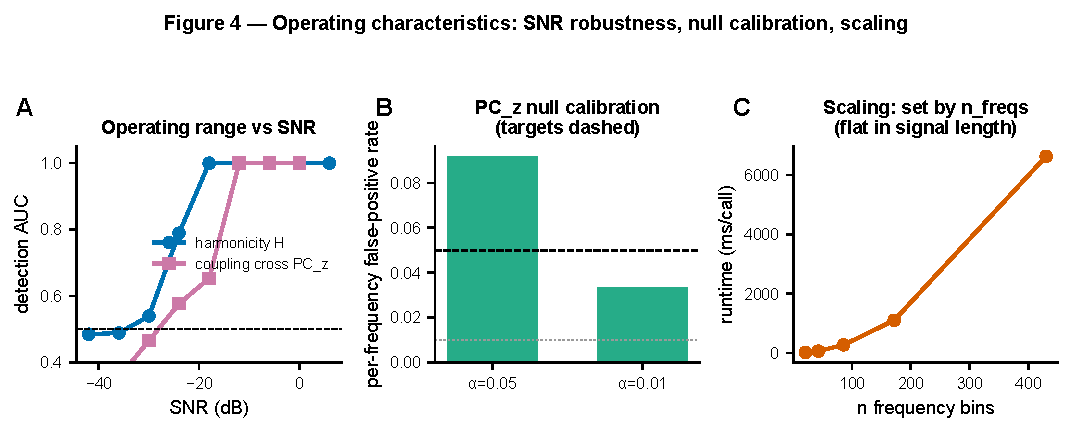
\includegraphics[width=\linewidth]{figures/method_Fig4_operating.pdf}
\caption{\textbf{Operating characteristics.} \textbf{(A)} Detection AUC vs signal-to-noise ratio for harmonicity $H$ and cross-signal coupling $\mathrm{PC}_z$ (chance dashed); $H$ holds to $\approx-18$~dB, coupling has a sharp threshold near $-12$~dB. \textbf{(B)} Null calibration of $\mathrm{PC}_z$ on uncoupled pairs (per-instance false-positive rate; $n=120$): mildly anti-conservative ($\approx0.09$ at $\alpha=0.05$). \textbf{(C)} Runtime is set by the frequency-grid size, not signal length.}
\label{fig:4}
\end{figure}

\subsection{Comparison with established measures}
A descriptor framework is only useful if it holds its own against the established measures it generalizes, so we benchmarked the two factors directly against field-standard baselines: the framework's phase-coupling factor against an oracle raw n:m phase-locking value (PLV), and the harmonicity factor against the classical harmonic-to-noise ratio (HNR). The comparison is deliberately demanding because the baselines are given an advantage the framework does not take: the oracle PLV is told the true n:m ratio in advance, whereas the framework must discover it.

For coupling detection, the surrogate-normalized phase-coupling factor $\mathrm{PC}_z$ matched the oracle raw n:m PLV across the usable signal-to-noise range, and was in fact \emph{more} robust as conditions degraded, reaching reliable detection roughly $6$ dB lower in SNR than the oracle baseline. This means the framework recovers the same coupling the gold-standard measure does, and then keeps detecting it after the gold-standard measure has failed -- while it does this without being handed the true ratio, instead auto-selecting the n:m relationship from the data, and while it returns a calibrated surrogate null that the raw PLV does not provide. The earlier saturation is therefore a practical gain: the same information is obtained from noisier or shorter data, and it arrives with a built-in significance reference.

For harmonicity, the framework's $H$ matched the classical HNR at usable SNR, with both reaching detection AUC $\approx 1.0$ at and above $-18$ dB. We are explicit about where HNR wins: at extreme SNR (below $-24$ dB) the single-scalar HNR is somewhat more noise-robust than $H$. The point of $H$ is not to out-detect HNR at its own one-number task but to do strictly more: $H$ returns a per-frequency harmonicity spectrum rather than a single number, extends naturally to multi-component and cross-signal settings, and scores inharmonicity explicitly rather than only the presence of a harmonic series. These are capabilities a scalar HNR structurally cannot offer.

Taken together (Figure 5), the baselines establish that the framework loses nothing relative to the standard tools on their home turf -- it ties or slightly beats them on detection -- while converting each scalar measure into an interpretable, per-frequency, null-calibrated, multi-signal-capable spectrum. The honest reading is parity-plus: equal detection, added structure and inference, with a single acknowledged exception at extreme low SNR where the classical HNR remains preferable.

\begin{figure}[t]\centering
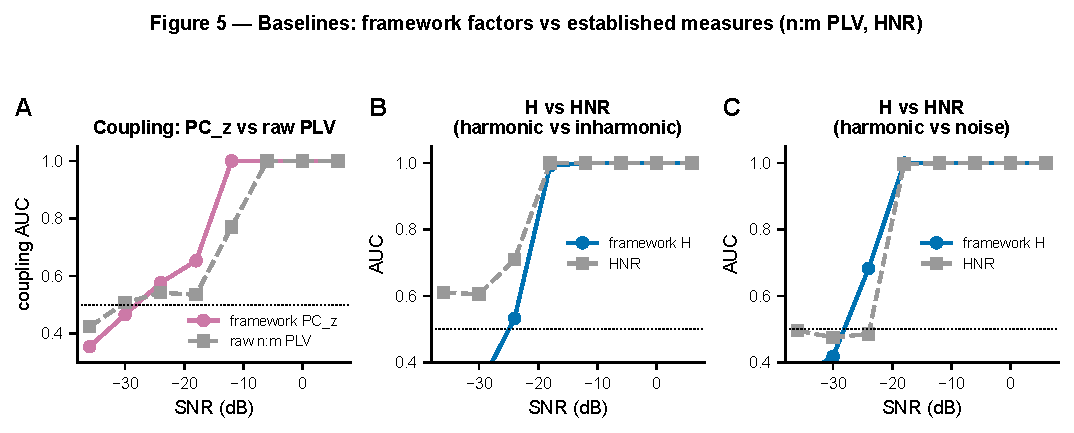
\includegraphics[width=\linewidth]{figures/method_Fig5_baselines.pdf}
\caption{\textbf{Comparison with established measures.} \textbf{(A)} Coupling detection: framework $\mathrm{PC}_z$ matches the oracle raw n:m phase-locking value and saturates $\approx6$~dB earlier. \textbf{(B,C)} Harmonicity $H$ vs the classical harmonic-to-noise ratio, separating harmonic from inharmonic (B) and from noise (C); $H$ matches HNR at usable SNR and adds a per-frequency spectrum.}
\label{fig:5}
\end{figure}

\subsection{Method choices and the locking mechanism}
Because the toolbox exposes its method choices as a swappable strategy registry, a user must decide which harmonic kernel and which coupling metric to use, and a natural worry is that this choice silently determines the result. We therefore asked whether the choice matters for accuracy, and, separately, whether the framework reproduces the dynamics it is meant to describe.

Sweeping the full registry on the recovery task, detection accuracy saturated: all twenty kernel$\times$metric configurations fell within $[0.982, 1.000]$. In other words, the framework is robust to method choice -- no combination materially out-detects another, and a user cannot accidentally pick a configuration that fails. With accuracy effectively fixed, the practical differentiator becomes runtime, and here the configurations differ sharply: the \texttt{harmsim} kernel ran about $27\times$ faster than \texttt{subharm\_tension} ($0.21$ s versus $5.64$ s per call) at equal accuracy. The recommendation that follows is concrete and evidence-based: default to the fast kernel, because the slow one buys no accuracy.

We then used the registry to perform a mechanistic sanity check against established nonlinear-dynamics theory. In a forced van der Pol oscillator -- a canonical mode-locking system -- we measured the width of each Arnold tongue, the range of forcing over which the oscillator locks to a given n:m ratio. Classical theory holds that simpler ratios lock over wider parameter ranges. The framework recovered exactly this dependence: Arnold-tongue width correlated negatively with ratio complexity ($\rho = -0.50$) and positively with the framework's own harmonicity factor ($\rho = +0.41$). The harmonicity factor thus tracks lockability the way synchronization theory predicts, which both validates $H$ as a meaningful quantity and supplies the physical reason why phase coupling is easier at simple ratios. We stress that this dependence is not a discovery: it is textbook synchronization theory (Arnold 1965; Pikovsky, Rosenblum \& Kurths 2001), used here purely as a construct-validity check that the framework behaves as a correct description of a known oscillator should (Figure 6).

\begin{figure}[t]\centering
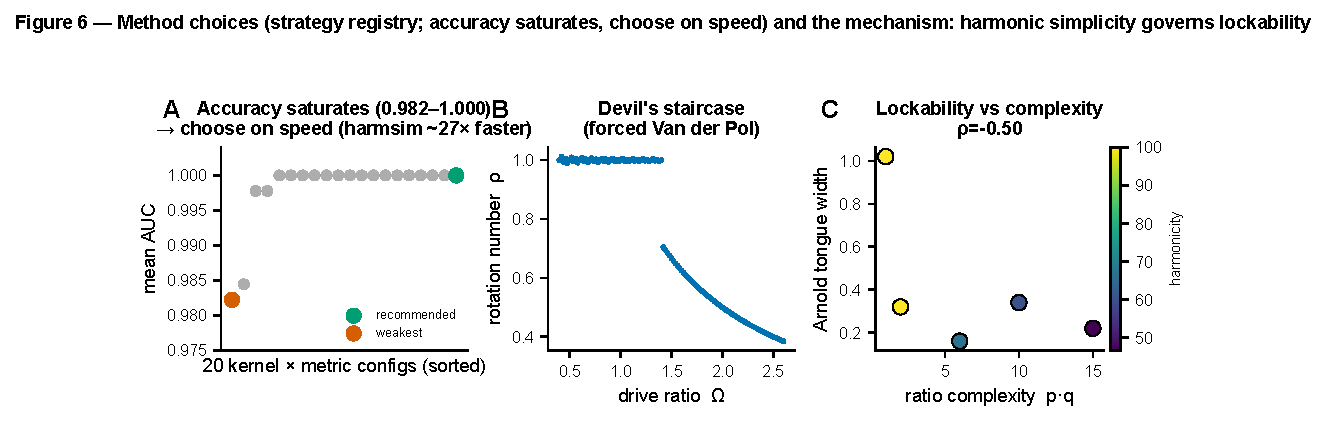
\includegraphics[width=\linewidth]{figures/method_Fig6_strategy_mechanism.pdf}
\caption{\textbf{Method choices and the locking mechanism.} \textbf{(A)} Across the strategy registry, detection accuracy saturates (all configurations $0.982$--$1.000$), so the practical choice is runtime (\texttt{harmsim} $\sim27\times$ faster). \textbf{(B)} Rotation number $\rho(\Omega)$ of a forced van der Pol oscillator. \textbf{(C)} Arnold-tongue width vs ratio complexity (colour: harmonicity), recovering the classical dependence of lockability on ratio simplicity ($\rho_s=-0.50$).}
\label{fig:6}
\end{figure}

\subsection{Application to real biosignals}
Synthetic validation shows the framework recovers structure it was built to find; the harder question is whether it produces interpretable, defensible results on real recordings. We evaluated it on human EEG and across signal modalities, holding it to honest baselines throughout and flagging confounds rather than claiming wins.

For a within-subject cortical-state contrast, eyes-open versus eyes-closed decoded at AUC $0.81$ under leave-one-subject-out cross-validation over ten subjects. Critically, this exactly matched a relative-alpha-power baseline (also $0.81$): the framework provides an interpretable harmonic-organization axis on this contrast, not an improvement over band power, and we report it as such. Examining the eyes-closed "more harmonic" effect more carefully exposed an important methodological point: the effect is $1/f$-dependent. With aperiodic removal, $H_{\max}$ decoded the contrast at AUC $0.83$; without it, decoding collapsed to $0.29$ -- worse than chance -- because the background $1/f$ slope, not genuine harmonic organization, was driving the raw difference. This is direct evidence that harmonicity differences must be read only after aperiodic removal.

A rest-run versus motor-run contrast reached AUC $0.62$ (permutation $p = 0.001$), modestly above a single-band-power baseline of $0.54$. We deliberately do not read this as a motor advantage: it is a run-level, baseline-versus-task comparison confounded by arousal and time-on-task, not a clean event-locked motor decode, and we state that limitation plainly rather than overinterpreting the gap.

Finally, the full feature vector fingerprinted seven signal modalities at $99\%$ accuracy ($4$-fold cross-validation, $0.99 \pm 0.02$; permutation $p = 0.005$; chance $14\%$). This is best read as a multivariate resonance signature on an intentionally easy separation -- a demonstration that the descriptors carry modality-specific information, not a claim of a hard discrimination problem solved (Figure 7). Across all of these, the consistent message is honest scope: the framework supplies an interpretable harmonic axis that ties band power on amplitude tasks, and its value lies in interpretability and in surfacing confounds such as the $1/f$ dependence, not in beating the simplest baseline.

\begin{figure}[t]\centering
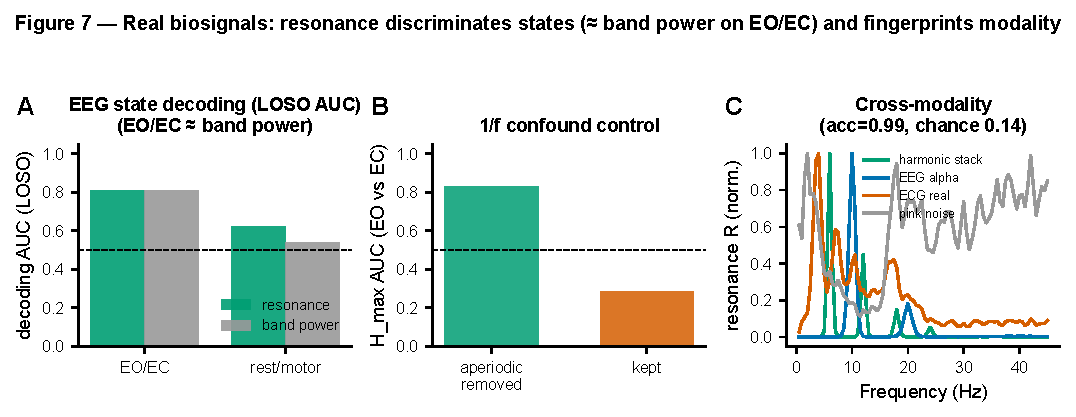
\includegraphics[width=\linewidth]{figures/method_Fig7_real_biosignals.pdf}
\caption{\textbf{Application to real biosignals.} \textbf{(A)} Leave-one-subject-out decoding AUC, resonance vs relative band power, for eyes-open/closed and a rest/motor contrast. \textbf{(B)} The eyes-closed harmonicity effect is aperiodic-dependent ($H$ AUC with vs without 1/f removal). \textbf{(C)} Normalized resonance spectra fingerprint seven signal modalities (cross-validated accuracy vs chance).}
\label{fig:7}
\end{figure}

\subsection{Network-level resonance connectivity}
The same resonance operator generalizes from a single signal to a channel$\times$channel matrix, allowing harmonic and phase-coupling structure to be read across an array of electrodes. To test whether this multichannel layer recovers true network structure, we planted a coupled cluster of channels in a synthetic montage and asked whether the cross-resonance connectivity matrix separates within-cluster pairs from the rest.

All three spectra recovered the planted cluster, with the phase-aware factors performing best: within-cluster versus rest separation reached AUC $0.74$ for $H$, $0.80$ for $\mathrm{PC}$, and $0.81$ for $R$. The structure of the matrices is informative in itself. The $H$ matrix was diffuse, because harmonicity is near-uniform within a shared-spectrum cluster and so blurs the cluster boundary; the $\mathrm{PC}$ matrix was sharper, isolating the coupled pairs more cleanly; and $R \approx \mathrm{PC}$, because where $H$ is near-uniform the product inherits its contrast from the phase factor. This recapitulates at the network level the single-signal result that $R$ is dominated by $H$ in absolute terms but reports coupling structure through $\mathrm{PC}$.

We are explicit about an important caveat. The scalar reducer used to collapse each channel pair to a single connectivity value is broadband and overlap-biased, so part of the recovered structure is driven by shared spectra rather than by pure cross-channel phase coupling. Isolating genuine n:m phase coupling above a power-preserving null requires the IAAFT surrogate-z variant, which retains the phase information that $H$ does not survive under a power-preserving surrogate. The connectivity layer therefore recovers coupled clusters reliably (Figure 8), but a user who needs \emph{pure} phase coupling -- as opposed to coupling plus shared spectral content -- must use the surrogate-z form rather than the raw scalar reducer.

\begin{figure}[t]\centering
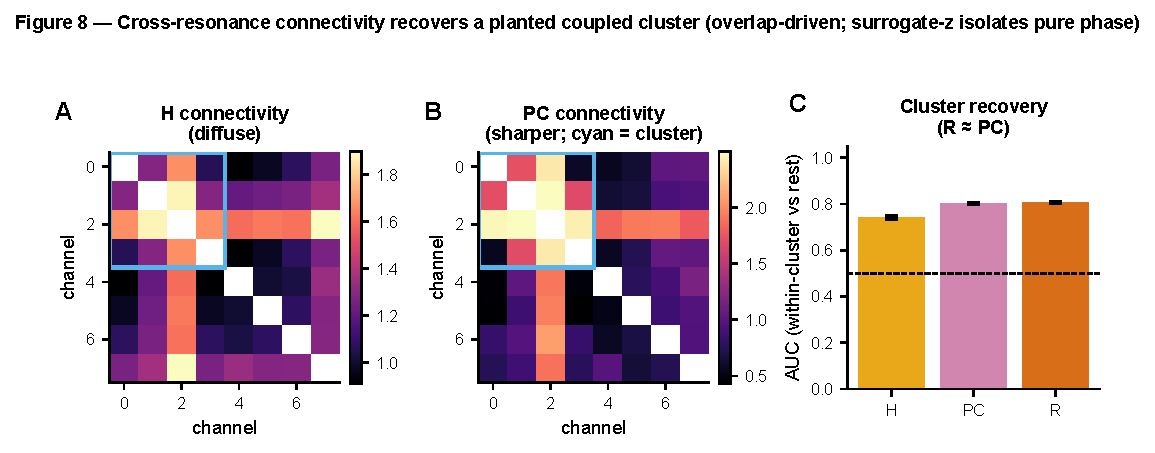
\includegraphics[width=\linewidth]{figures/method_Fig8_connectivity.pdf}
\caption{\textbf{Network-level resonance connectivity.} \textbf{(A,B)} Cross-resonance connectivity matrices (harmonicity, phase coupling) for a montage with a planted coupled cluster (cyan box); $H$ is diffuse, $\mathrm{PC}$ sharper. \textbf{(C)} Within-cluster-vs-rest recovery AUC ($H$ 0.74, $\mathrm{PC}$ 0.80, $R$ 0.81); recovery is overlap-driven, and isolating pure phase requires the IAAFT surrogate-z variant.}
\label{fig:8}
\end{figure}

\subsection{Spectral-complexity descriptors as features}
A scalar summary of a spectrum, such as its mean, throws away the shape of the spectrum -- yet the shape is often what distinguishes one signal class from another. We therefore treat a panel of complexity descriptors computed \emph{of} the $H$, $\mathrm{PC}$, and $R$ spectra -- spectral flatness, entropy, spread, and Higuchi fractal dimension -- as first-class features in their own right, and asked whether they carry information the scalar summaries discard.

On signals of known structure, these descriptors formed a distinctive per-class "resonance fingerprint": each signal type occupies a characteristic region of descriptor space, so the shape of its resonance spectra, not just their average level, identifies it. The clearest demonstration of the added information is a case where the scalar summary fails outright. The mean harmonicity $H_{\mathrm{avg}}$ conflated four very different signal classes -- pure tone, inharmonic, narrowband, and pink noise -- assigning all of them essentially the same value ($\approx 0.17$), so an analyst relying on mean $H$ alone would see them as indistinguishable. The spectral flatness of the $H$ spectrum, by contrast, separated exactly these classes, spreading them from $0.17$ to $0.93$ and yielding a harmonic-versus-noise separation of AUC $1.0$.

The interpretation is that the resonance \emph{spectra} encode discriminative structure in their distribution across frequency that any single reduction averages away, and the descriptors recover it cheaply. Rather than committing to one scalar summary and hoping it captures the relevant contrast, a user can report the full descriptor fingerprint and let class differences in spectral shape -- flatness, entropy, spread, fractal dimension -- surface differences that the mean conflates (Figure 9). The descriptors are thus not decorative add-ons but a substantive part of what the framework offers: a multivariate, interpretable readout of resonance-spectrum shape that complements the scalar factors.

\begin{figure}[t]\centering
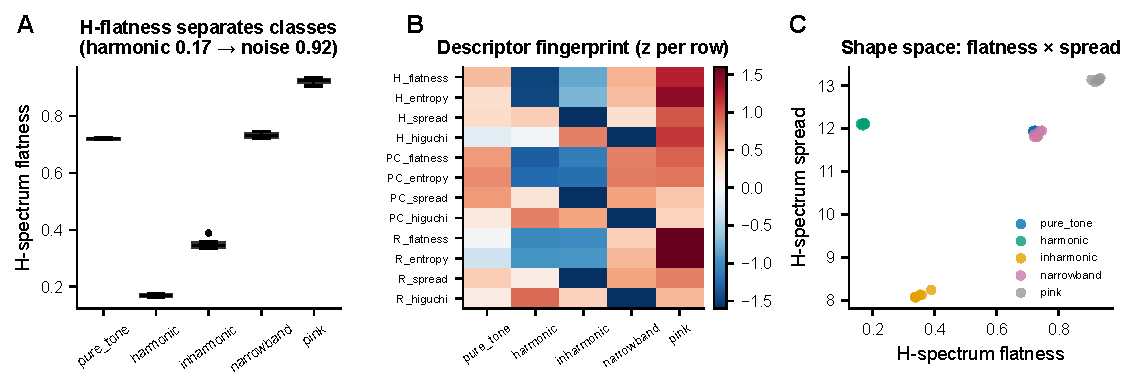
\includegraphics[width=\linewidth]{figures/method_Fig9_descriptors.pdf}
\caption{\textbf{Spectral-complexity descriptors of the resonance spectra.} \textbf{(A)} Spectral flatness of the $H$ spectrum by signal class. \textbf{(B)} Per-class descriptor fingerprint (z-scored across classes). \textbf{(C)} Shape space (flatness $\times$ spread); the descriptors carry information the scalar summaries miss.}
\label{fig:9}
\end{figure}

\section{Discussion}
We set out to make harmonic organization a measurable, reportable, and comparable property of biological time series, and to do so in a way that separates two things that are often conflated. The framework decomposes a signal into a per-frequency harmonicity spectrum $H(f)$, which scores how closely spectral peaks sit at integer ratios; a per-frequency phase-coupling spectrum $\mathrm{PC}(f)$, which scores how stably oscillatory components hold an $n{:}m$ phase relation; and their product $R = H\cdot\mathrm{PC}$. Across synthetic ground truth we showed that these are genuinely separable axes rather than two views of one quantity: harmonicity is \emph{exactly} phase-blind ($\rho(H,\kappa) = 0.00$), responding only to ratio complexity, while phase coupling tracks locking strength (Figure 1). The product is the principled conjunction of the two. When harmonicity and phase locking are varied as independent latent factors, a conjunction separates a true resonance from single-factor confounds far better than either factor alone (specificity AUC $\approx 0.99$ for conjunctions versus $\leq 0.76$ for $H$ or $\mathrm{PC}$ singly and $0.66$ for the OR-disjunction), and $R$ adds a phase-coherence requirement that $H$ lacks: phase-scrambling a harmonic signal leaves its power spectrum and therefore $H$ untouched (AUC $0.50$) while $R$ collapses to chance-discrimination of the scramble (AUC $1.00$) (Figure 2). On synthetic ladders and planted $n{:}m$ locks the framework recovers known structure with high fidelity (harmonic-richness $\rho = 0.98$; coupling AUC $\approx 1.0$; Figure 3), degrades gracefully with decreasing signal-to-noise ratio (Figure 4), is competitive with established single-purpose measures (Figure 5), recovers the textbook dependence of lockability on ratio complexity (Figure 6), discriminates real EEG states and fingerprints physiological modalities (Figure 7), extends to multichannel connectivity (Figure 8), and yields spectral-complexity descriptors that carry information the scalar summaries discard (Figure 9). The result is a single operator that turns harmonic organization into an interpretable, per-frequency, honestly-scoped descriptor with single-signal, cross-signal, and connectivity forms.

It is important to be precise about where the novelty lies, because much of what the framework rests on is established. The harmonicity construct itself has a long lineage in audio analysis, music-information retrieval, and music perception, and the specific number-theoretic ratio kernels we use are inherited rather than introduced. That harmonic organization is a \emph{separable} factor — and a confound for cross-frequency coupling when waveforms are non-sinusoidal — is prior art (Dellavale et al. 2020; Aru et al. 2015), as is the broader observation that non-sinusoidal structure can masquerade as coupling. The $n{:}m$ phase-synchronization estimators are standard, and the synchronization theory that explains our coupling results — the Arnold-tongue narrowing in which complex ratios require stronger coupling to lock, and the leading-order $a_n\cdot a_m$ coupling strength of weakly coupled phase oscillators — is recovered here from textbook nonlinear dynamics (Arnold; Pikovsky, Rosenblum \& Kurths), not discovered. We reproduce these effects deliberately, as construct validation. What is new is the integration: a swappable strategy registry that crosses harmonicity kernels with $n{:}m$ phase-\emph{phase} coupling metrics and combine rules, making the method choice an explicit and testable variable; the reusable per-frequency $R = H\cdot\mathrm{PC}$ descriptor that reports both factors and their conjunction as separate spectra; factor-level surrogate inference; and cross-signal and connectivity generalizations of the same operator. The toolboxes that share this swappable-metric, surrogate-normalized software pattern target phase-\emph{amplitude} coupling, so no off-the-shelf equivalent for an $n{:}m$ phase-phase resonance exists. The contribution, in short, is unification, validation, and tooling around constructs that the field already holds to be real.

Two methodological cautions emerge that generalize well beyond this particular toolbox. The first concerns the aperiodic background. On pure colored noise, spectral harmonicity rises monotonically with the $1/f$ slope, so any comparison that attributes a harmonicity \emph{difference} to a change in oscillatory organization is confounded whenever the conditions also differ in their broadband spectral tilt. This is not a hypothetical worry: the eyes-closed "more harmonic" effect in real EEG was strongly $1/f$-dependent, with $H_{\max}$ discriminating eyes-open from eyes-closed at AUC $0.83$ after aperiodic removal but only $0.29$ without it. We therefore treat aperiodic removal as mandatory whenever a harmonicity difference is interpreted across conditions that may differ in background $1/f$. The second caution concerns where inference is applied. Because $R$ is dominated by $H$ and $H$ is fixed by the power spectrum, a surrogate test on the composite $R$ under a power-preserving null is effectively a test on the PSD and can mask a genuine phase-coupling effect carried by $\mathrm{PC}$. Inference must target the factor that carries the effect — $\mathrm{PC}_z$ for $n{:}m$ coupling — rather than a composite dominated by another factor. This is a concrete, operational instance of the broader lesson from the phase-phase-coupling-inflation literature (Scheffer-Teixeira \& Tort 2016) that such claims are easily inflated by mismatched statistics, and it motivates our factor-level, aperiodic-corrected, surrogate-normalized design.

It is equally important to be clear about what the framework is for and what it is not. It supplies an interpretable harmonic and cross-frequency-coupling axis: a way to ask, per frequency, how harmonically organized a signal is and how stably its components are phase-locked, with a decomposition $\log R = \log H + \log \mathrm{PC}$ that attributes a weak resonance to its cause. It is \emph{not} a replacement for band power. On single-band amplitude tasks the framework matches rather than beats band power — eyes-open versus eyes-closed decoded at AUC $0.81$, identical to a relative-alpha-power baseline — and we present it as an interpretable complement, not a more powerful classifier. The near-ceiling AUCs ($\approx 1.0$) reported on synthetic data should be read accordingly. They index construct validity on ground truth where the planted effect is, by design, strong and isolated; they are not estimates of the magnitude of harmonic coupling in real biosignals, where the effects we observed were modest and reported as such. The full-feature modality fingerprint (seven modalities at $99\%$) is best read as a multivariate signature on an intentionally easy separation rather than as evidence of subtle coupling.

Several limitations bound the present work and point toward its extensions. The phase estimator is currently STFT-only; Hilbert and wavelet estimators occupy registry slots but remain to be validated, and a time-resolved estimator would be the natural route to non-stationary and event-locked analyses. The phase-coupling surrogate null is mildly anti-conservative, with a per-instance false-positive rate of $\approx 0.09$ at $\alpha = 0.05$ on uncoupled pairs, so strict type-I control calls for more surrogates or a multiple-surrogate correction. The scalar connectivity reducer is broadband and overlap-biased, so cluster recovery in the connectivity matrix ($R \approx \mathrm{PC}$, within-cluster AUC up to $0.81$) is driven partly by shared spectra; isolating \emph{pure} cross-channel phase coupling above a PSD-preserving null requires the IAAFT surrogate-$z$ variant, since $H$ does not survive a power-preserving surrogate. And because the rest-versus-motor EEG contrast is a run-level, baseline-versus-task comparison confounded by arousal and time-on-task, the modest advantage there (AUC $0.62$ versus $0.54$) should not be read as a genuine motor-decoding result. None of these caveats undercut the central claim. Harmonicity and phase coupling are separable axes worth measuring and reporting as distinct per-frequency spectra, and their product is a principled, interpretable conjunction. With those foundations in place, the descriptor is positioned as a general-purpose lens on harmonic organization — one that opens naturally toward tracking dynamic state, characterizing developmental change, and probing clinical conditions in which the harmonic and cross-frequency-coupling structure of physiological rhythms is itself the question of interest.

\section{Methods}
\textbf{Overview of the resonance computation.} The framework decomposes a time series into two per-frequency factors and their product. For a power spectrum $p(f)$, a harmonic kernel $S[i,j]$ scores how close each pair of frequencies sits to a simple integer ratio, and a phase-coupling kernel scores how stably the corresponding spectral components hold an $n$:$m$ phase relation. PSD-weighted reductions over all partner frequencies collapse these pairwise scores into two spectra,
\[
H(f_i) = p(f_i)\cdot\sum_j S[i,j]\,p(f_j),\qquad
\mathrm{PC}(f_i) = p(f_i)\cdot\sum_j W[i,j]\,\Phi[i,j]\,p(f_j),
\]
where $H$ is the \emph{harmonicity} spectrum (how harmonically organized the spectrum is at each frequency), $\mathrm{PC}$ is the \emph{phase-coupling} spectrum (how stably components hold an $n$:$m$ phase relation), and their product $R(f) = H(f)\cdot\mathrm{PC}(f)$ is the \emph{resonance} spectrum. Single-signal analyses ran through the \texttt{compute\_resonance} pipeline, which estimates phase with a short-time Fourier transform (STFT), performs the per-frequency factor reduction above, and combines the factors with a product rule. Cross-signal and multichannel analyses used \texttt{compute\_cross\_resonance} and \texttt{compute\_cross\_resonance\_connectivity}, which apply the identical operator to phases estimated from two signals or from each pair of channels. Unless noted, the analysis band was $2-45$ Hz at $0.5$ Hz spectral resolution (extended to $0.5-45$ Hz for ECG, where low-frequency harmonics carry the QRS series). The recommended configuration pairs the \texttt{harmsim} harmonic kernel and the \texttt{fraction} ratio kernel with the convention-correct \texttt{nm\_plv\_canonical} coupling metric. Each spectrum was additionally summarized by a panel of complexity descriptors (mean, maximum, spectral flatness, entropy, spectral spread, Higuchi fractal dimension, and peak-harmonic-similarity), treated as first-class features.

\textbf{What the coupling is measured on.} The phase-coupling factor is a phase$-$phase, polyrhythmic quantity computed between \emph{pairs of spectral components}, and it is important to distinguish it from the more familiar coherence and phase$-$amplitude measures. The STFT phase estimator returns the instantaneous phase $\theta(f,t)$ at each frequency bin; for a pair of bins $f_i,f_j$ the ratio kernel selects the nearest rational $n$:$m$ approximating $f_j/f_i$, and the coupling metric measures how consistently the generalized phase difference $n\cdot\theta_i - m\cdot\theta_j$ stays fixed over time. Because the comparison is between two phases at a rational frequency ratio, this detects $n$:$m$ (polyrhythmic) phase relations between oscillatory components rather than the special case of $1$:$1$ phase coherence, and it does not involve amplitude at all, so it is distinct from phase$-$amplitude coupling. The same operator was evaluated in three regimes: \emph{within a signal}, where the coupling is cross-frequency coupling between the signal's own peaks and yields the $\mathrm{PC}(f)$ spectrum; \emph{between two signals}, via \texttt{compute\_cross\_resonance}; and \emph{across channels}, where pairwise application builds the $n_{\mathrm{elec}}\times n_{\mathrm{elec}}$ connectivity matrix. The available coupling metrics span the phase-locking value and the volume-conduction-robust phase-lag family (\texttt{nm\_plv}, \texttt{nm\_plv\_canonical}, \texttt{nm\_pli}, \texttt{nm\_wpli}, \texttt{nm\_rrci}); the harmonic and ratio kernels (\texttt{harmsim}, \texttt{subharm\_tension}; \texttt{binary}, \texttt{fraction}) and combine rules (\texttt{product}, \texttt{geomean}, \texttt{harmmean}, \texttt{min}, \texttt{weighted\_log}) are likewise swappable through the strategy registry, making each method choice an explicit, testable variable.

\textbf{Surrogate inference at the factor level.} Significance was assessed by comparing an observed spectrum to an ensemble of phase-randomizing surrogates and forming a per-frequency $z$-score. For single signals we used amplitude-adjusted Fourier-transform (AAFT) surrogates, which preserve the power spectrum and amplitude distribution while destroying phase relations; for cross-channel inference we used the iterated variant (IAAFT), which preserves the spectra of both members of a pair. A central practical point determined how the $z$-score must be applied: we $z$-scored \emph{each factor ($H$, $\mathrm{PC}$, and $R$) separately} against the same surrogate ensemble, and inference for coupling targets $\mathrm{PC}_z$ rather than the composite $R$. The reason is that $R$ is $H$-dominated and therefore essentially PSD-driven under a power-preserving null; testing $R$ can mask a genuine coupling effect that lives in $\mathrm{PC}$. The phase-coupling factor is the correct detector for $n$:$m$ coupling and must be read as $\mathrm{PC}_z$, not in absolute terms. Surrogate counts were $40-150$ per analysis (more under the paper-grade pass).

\textbf{Aperiodic removal is mandatory across conditions.} On pure colored noise, harmonicity rises monotonically with the $1/f$ slope, a confound for any spectral harmonicity measure. Whenever the conditions being compared could differ in their background $1/f$, we therefore removed the aperiodic component before computing $H$ (\texttt{remove\_aperiodic=True}). Removal fits a two-parameter power law $P(f) = a\cdot f^{b}$ to the PSD over the analysis band by non-linear least squares and subtracts it. This is a deliberately lightweight aperiodic correction and is \emph{not} a FOOOF/specparam-style periodic/aperiodic peak decomposition; it removes only the broadband $1/f$ trend so that condition differences in harmonicity cannot be attributed to differences in spectral slope.

\textbf{Signals and data provenance.} Validation used synthetic generators with known structure together with real biosignals. The synthetic generators produced harmonic ladders, $n$:$m$ phase locks, polyrhythms, inharmonic and noise controls, and a grid that independently varies harmonicity and phase coupling, all placed on a matched $1/f$ background (sampling $250-500$ Hz, durations $12-40$ s, with SNR and random-seed grids varied per analysis). Real EEG came from the PhysioNet EEG Motor Movement/Imagery database (eegmmidb), auto-fetched via \texttt{mne.datasets.eegbci} for subjects $1-10$. We formed an eyes-open versus eyes-closed contrast from the two baseline runs over occipital channels and a rest versus motor contrast from a baseline run versus a motor-execution run over central channels, band-pass filtered $1-45$ Hz at the native $160$ Hz sampling rate. ECG, PPG, and respiration signals were simulated with neurokit2, supplemented by one bundled real ECG clip tiled to length (noted where used). No data are redistributed; the EEG is downloaded on first run and the physiological signals are generated locally.

\textbf{Default analysis parameters.} Unless overridden through the registry, analyses used $0.5$ Hz spectral resolution over a $2-45$ Hz band ($0.5-45$ Hz for ECG), the \texttt{harmsim} harmonic kernel, the \texttt{fraction} ratio kernel with a maximum denominator of $16$, the \texttt{nm\_plv\_canonical} coupling metric, the \texttt{product} combine rule, and aperiodic removal enabled. STFT overlap was set per analysis.

\textbf{Statistics.} Detection and discrimination were scored by rank area under the curve (Mann$-$Whitney; $0.5 = $ chance), with percentile bootstrap $95\%$ confidence intervals ($2000-3000$ resamples at a fixed seed). EEG decoding used leave-one-subject-out cross-validation, so that no subject contributed to both training and test folds. Where stated, permutation tests provided exact $p$-values by relabeling.

\textbf{Reproducibility note.} The core engine is biotuner, pinned to the immutable commit \texttt{fc158c3} (full SHA recorded in \texttt{requirements.txt}). This pin is load-bearing: the PyPI 0.4.1 build predates a phase-row alignment fix and silently breaks cross-frequency coupling detection at $f_{\min} \geq 1$ Hz. Because the version string is uninformative ($\texttt{biotuner.\_\_version\_\_}$ reads 0.4.1 even on the development branch), we pin the commit SHA rather than rely on a version check. The full numeric suite is reproduced with \texttt{python -m resonance\_paper.run\_all --paper} and all figures regenerated with \texttt{python -m resonance\_paper.paper.make\_method\_figures}.

\section*{References}
\begingroup\small
\begin{list}{}{\setlength{\itemsep}{1pt}\setlength{\leftmargin}{1.2em}\setlength{\itemindent}{-1.2em}}
\item Arnold, V. I. (1965). Small denominators I: mappings of the circle onto itself. \emph{AMS Transl. Ser. 2}, 46, 213–284.
\item Aru, J., Aru, J., Priesemann, V., Wibral, M., Lana, L., Pipa, G., Singer, W., \& Vicente, R. (2015). Untangling cross-frequency coupling in neuroscience. \emph{Curr. Opin. Neurobiol.}, 31, 51–61.
\item Bellemare-Pepin, A., \& Jerbi, K. (2025). Biotuner: a Python toolbox integrating music theory and signal processing for harmonic analysis of physiological and natural time series. \emph{Brain Informatics}, 12.
\item Bidelman, G. M. (2013). The role of the auditory brainstem in processing musically relevant pitch. \emph{Front. Psychol.}, 4, 264.
\item Bidelman, G. M., \& Krishnan, A. (2009). Neural correlates of consonance, dissonance, and the hierarchy of musical pitch in the human brainstem. \emph{J. Neurosci.}, 29(42), 13165–13171.
\item Boersma, P. (1993). Accurate short-term analysis of the fundamental frequency and the harmonics-to-noise ratio of a sampled sound. \emph{IFA Proc.}, 17, 97–110.
\item Boremanse, A., Norcia, A. M., \& Rossion, B. (2013). An objective signature for visual binding of face parts in the human brain. \emph{J. Vis.}, 13(11), 6.
\item Bowling, D. L., \& Purves, D. (2015). A biological rationale for musical consonance. \emph{PNAS}, 112(36), 11155–11160.
\item Canolty, R. T., et al. (2006). High gamma power is phase-locked to theta oscillations in human neocortex. \emph{Science}, 313, 1626–1628.
\item Combrisson, E., et al. (2020). Tensorpac: an open-source Python toolbox for tensor-based phase-amplitude coupling measurement. \emph{PLOS Comput. Biol.}, 16(10), e1008302.
\item Daido, H. (1996). Onset of cooperative entrainment in limit-cycle oscillators. \emph{Physica D}, 91, 24–66.
\item Dellavale, D., Urdapilleta, E., Cámpora, N., Velarde, O. M., Kochen, S., \& Mato, G. (2020). Spectral harmonicity and cross-frequency coupling in nonlinear oscillators and biologically plausible neural network models. \emph{Phys. Rev. E}, 102, 062401.
\item Donoghue, T., et al. (2020). Parameterizing neural power spectra into periodic and aperiodic components. \emph{Nat. Neurosci.}, 23, 1655–1665.
\item Dupré la Tour, T., et al. (2017). Non-linear auto-regressive models for cross-frequency coupling in neural time series (pactools). \emph{PLOS Comput. Biol.}, 13(12), e1005893.
\item Ermentrout, G. B., \& Kopell, N. (1991). Multiple pulse interactions and averaging in systems of coupled neural oscillators. \emph{J. Math. Biol.}, 29, 195–217.
\item Gill, K. Z., \& Purves, D. (2009). A biological rationale for musical scales. \emph{PLoS ONE}, 4(12), e8144.
\item Glass, L., \& Mackey, M. C. (1988). \emph{From Clocks to Chaos: The Rhythms of Life.} Princeton Univ. Press.
\item Gramfort, A., et al. (2013). MEG and EEG data analysis with MNE-Python. \emph{Front. Neurosci.}, 7, 267.
\item Harrison, P. M. C., \& Pearce, M. T. (2020). Simultaneous consonance in music perception and composition. \emph{Psychol. Rev.}, 127(2), 216–244.
\item Johnston, J. D. (1988). Transform coding of audio signals using perceptual noise criteria. \emph{IEEE JSAC}, 6(2), 314–323.
\item Kuramoto, Y. (1984). \emph{Chemical Oscillations, Waves, and Turbulence.} Springer.
\item Lachaux, J.-P., Rodriguez, E., Martinerie, J., \& Varela, F. J. (1999). Measuring phase synchrony in brain signals. \emph{Hum. Brain Mapp.}, 8, 194–208.
\item Large, E. W., Kim, J. C., Flaig, N. K., Bharucha, J. J., \& Krumhansl, C. L. (2016). A neurodynamic account of musical tonality. \emph{Music Percept.}, 33(3), 319–331.
\item Lee, K. M., Skoe, E., Kraus, N., \& Ashley, R. (2009). Selective subcortical enhancement of musical intervals in musicians. \emph{J. Neurosci.}, 29(18), 5832–5840.
\item Lerud, K. D., Almonte, F. V., Kim, J. C., \& Large, E. W. (2014). Mode-locking neurodynamics predict human auditory brainstem responses to musical intervals. \emph{Hear. Res.}, 308, 41–49.
\item McDermott, J. H., Lehr, A. J., \& Oxenham, A. J. (2010). Individual differences reveal the basis of consonance. \emph{Curr. Biol.}, 20(11), 1035–1041.
\item Norcia, A. M., Appelbaum, L. G., Ales, J. M., Cottereau, B. R., \& Rossion, B. (2015). The steady-state visual evoked potential in vision research: a review. \emph{J. Vis.}, 15(6), 4.
\item Palva, J. M., Palva, S., \& Kaila, K. (2005). Phase synchrony among neuronal oscillations in the human cortex. \emph{J. Neurosci.}, 25(15), 3962–3972.
\item Pikovsky, A., Rosenblum, M., \& Kurths, J. (2001). \emph{Synchronization: A Universal Concept in Nonlinear Sciences.} Cambridge Univ. Press.
\item Plomp, R., \& Levelt, W. J. M. (1965). Tonal consonance and critical bandwidth. \emph{J. Acoust. Soc. Am.}, 38, 548–560.
\item Rodriguez-Larios, J., Bracho, A., \& Alaerts, K. (2019). Harmonic relationships between theta and alpha peaks facilitate cognitive performance. \emph{J. Neurosci.}, 39(32), 6291–6298.
\item Schalk, G., McFarland, D. J., Hinterberger, T., Birbaumer, N., \& Wolpaw, J. R. (2004). BCI2000: a general-purpose brain–computer interface system. \emph{IEEE Trans. Biomed. Eng.}, 51(6), 1034–1043. (PhysioNet eegmmidb)
\item Scheffer-Teixeira, R., \& Tort, A. B. L. (2016). On cross-frequency phase-phase coupling between theta and gamma oscillations in the hippocampus. \emph{eLife}, 5, e20515.
\item Schreiber, T., \& Schmitz, A. (1996). Improved surrogate data for nonlinearity tests. \emph{Phys. Rev. Lett.}, 77, 635–638.
\item Sethares, W. A. (1993). Local consonance and the relationship between timbre and scale. \emph{J. Acoust. Soc. Am.}, 94, 1218–1228.
\item Stam, C. J., Nolte, G., \& Daffertshofer, A. (2007). Phase lag index. \emph{Hum. Brain Mapp.}, 28, 1178–1193.
\item Stolzenburg, F. (2015). Harmony perception by periodicity detection. \emph{J. Math. Music}, 9(3), 215–238.
\item Tass, P., et al. (1998). Detection of n:m phase locking from noisy data: application to magnetoencephalography. \emph{Phys. Rev. Lett.}, 81, 3291–3294.
\item Terhardt, E., Stoll, G., \& Seewann, M. (1982). Algorithm for extraction of pitch and pitch salience from complex tonal signals. \emph{J. Acoust. Soc. Am.}, 71, 679–688.
\item Theiler, J., Eubank, S., Longtin, A., Galdrikian, B., \& Farmer, J. D. (1992). Testing for nonlinearity in time series: the method of surrogate data. \emph{Physica D}, 58, 77–94.
\item Tort, A. B. L., Komorowski, R., Eichenbaum, H., \& Kopell, N. (2010). Measuring phase-amplitude coupling between neuronal oscillations of different frequencies. \emph{J. Neurophysiol.}, 104, 1195–1210.
\item Vinck, M., et al. (2010). The pairwise phase consistency: a bias-free measure of rhythmic neuronal synchronization. \emph{NeuroImage}, 51, 112–122.
\item Vinck, M., et al. (2011). An improved index of phase-synchronization (wPLI). \emph{NeuroImage}, 55, 1548–1565.
\end{list}\endgroup

\end{document}